\def\equalfootnote{\mathrel{\ensurestackMath{\stackon[1pt]{=}{\footnotemark[0]}}}}
%//==============================--@--==============================//%
\label{sec:mechanics}
\subsection[3.1 Sistemas Mecânicos de Translação]{$\rightarrow$ Sistemas Mecânicos de Translação}
\label{sec:mechanics-translation}

``The cornerstone for obtaining a mathematical model, or the dynamic equations, for any mechanical system is Newton's law
$$
    \boxed{F = \frac{dp}{dt} = \frac{d}{dt} (m v) \equalfootnote ma}
$$
\noindent where:
\begin{itemize}
    \item $F$ = the vector sum of all forces applied to each body in a system, newtons (N),
    \item $p$ = linear momentum/translational momentum (kg ms$^{-1}$),
    \item $v$ = velocity (ms$^{-1}$), the directional speed of an object in motion as an indication of its rate of change in position as observed from a particular frame of reference,
    \item $a$ = the vector acceleration of each body with respect to an inertial reference frame (that is, one that is neither accelerating nor rotating with respect to the stars); often called inertial acceleration, ms$^{-2}$,
    \item $m$ = mass of the body, kg.''\cite{FranklinPowell2015}
\end{itemize}

\footnotetext[0]{Para uma massa invariante no tempo, ou aproximadamente constante.}

\phantomsection\addcontentsline{toc}{subsubsection}{3.1.1 Relações fundamentais baseadas em princípios físicos}
\renewcommand*{\thefootnote}{\fnsymbol{footnote}}
\begin{theo}[\underline{Molas Elásticas}]{def:Molas Elásticas}\label{def:MolasElásticas}
Quando uma mola é comprimida ou esticada, reage com uma força que se opõe à compressão (ou à extensão). Força desta que, para molas lineares, é dada por:
$$
    f = -kx
$$
Onde $k$ é a constante de Hooke [N/m].
\end{theo}

\begin{theo}[\underline{Atrito Viscoso}]{def:Atrito Viscoso}\label{def:AtritoViscoso}
Elemento que dissipa energia. Quando existe uma diferença de velocidade entre dois corpos o atrito corresponde a uma força que contraria o movimento. No caso linear, o atrito é dado por:
$$
    f = -\beta\dot{x}\ = -\beta v 
$$
\end{theo}

\mdfsetup{linewidth=2pt}
\begin{mdframed}
\textbf{Nota} $\rightarrow$ \textbf{Atrito estático} 

\noindent 
``Static friction is also known as stiction and models the fact that in some cases the friction
force is larger in magnitude for zero velocity than for a non-zero velocity. According to
the stiction model the system sticks if the velocity is zero and $|F_t | < F_s$, and it breaks
away if $|F_t | = F_s$ where $F_s > F_a$''\cite{Egeland2002}
\end{mdframed}

%//==============================--@--==============================//%
\clearpage
\subsection[3.2 Sistemas Mecânicos de Rotação]{$\rightarrow$ Sistemas Mecânicos de Rotação}
\label{sec:mechanics-rotation}

O \underline{Momento de Inércia} é o análogo da massa para a rotação. Quando um corpo em rotação com um \underline{Momento de Inércia} $J$ $[$Nms$^{2}]$ é atuado por um \underline{Binário} $T$ $[$Nm$]$, adquire aceleração angular dada por
$$
    \boxed{J\ddot{\theta} = T}
$$


\begin{theo}[\underline{Molas Elásticas}]{def:Mola Elástica de Rota}\label{def:MolaElasticaRota}
Quando a mola é desviada um ângulo $\theta$  em relação à posição de repouso, reage
com um binário que se opõe ao movimento, dada para molas lineares por:
$$
    T = -K\dot{\theta}\ 
$$
Onde $k$ é a "constante da mola" [Nm/rads$^{-1}$].
\end{theo}

\begin{theo}[\underline{Atrito Viscoso}]{def:Atrito Viscoso Rotação}\label{def:AtritoViscosoRotação}
Elemento que dissipa energia. Quando existe uma diferença de velocidade de rotação entre dois corpos o atrito corresponde a uma binário que contraria o movimento e que depende da velocidade angular. No caso linear, o atrito é dado por:
$$
    T = -\beta\dot{\theta}\ = -\beta \omega
$$
\end{theo}

\begin{theo}[\underline{Caixa de desmultiplicação}]{def:Caixa D}\label{def:Caixa D}
Uma caixa de desmultiplicação transforma o binário e a velocidade angular de acordo com as seguintes relações:
$$
    \omega_1 = \frac{1}{a}\omega_1\qquad
    T_1 = aT_2\qquad
    T_1 \omega_1 = T_2 \omega_2
$$

Onde $a = \frac{\omega_1}{\omega_2}$ é o inverso da razão de desmultiplicação da caixa.
\end{theo}




\begin{theo}[\underline{Transformação da rotação em translação}]{def:rotation-to-translation}\label{def:rotation-to-translation}
Assumindo que não existe escorregamento, nem perdas energéticas, temos
$$
    v = \omega r,\qquad F = \frac{1}{r} T
$$
\vspace{-1em}
\begin{figure}[H]
    \centering
    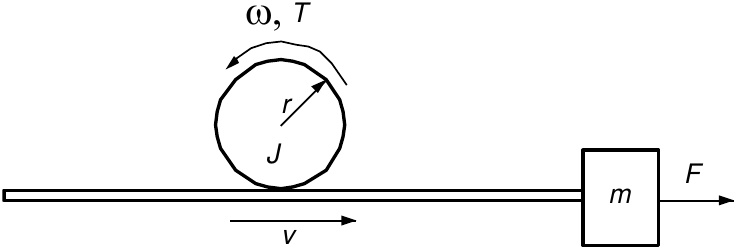
\includegraphics[width = 0.6\linewidth]{img/mechanics/convertion.png}
    \label{fig:convertion}
\end{figure}
\end{theo}

% \begin{figure}[H]
%     \centering
%     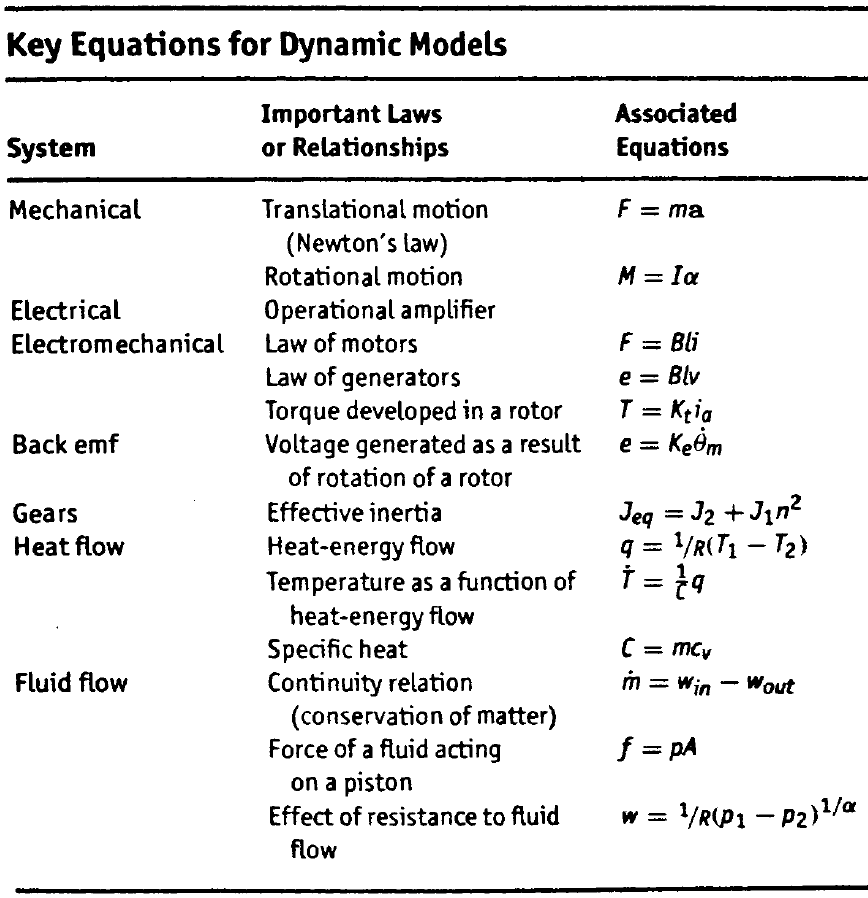
\includegraphics[width = 0.7\linewidth]{img/mechanics/key-equations.png}
%     \caption{Equações chave. \textbf{\underline{Nota:}} $M = I \alpha \iff J\ddot{\theta} = T$}
%     \label{fig:key-equations}
% \end{figure}
%//==============================--@--==============================//%
\newpage
\subsubsection[3.2.2 Motor Corrente Contínua]{$\rightarrow$ Motor de Corrente Contínua}
\mdfsetup{linewidth=2pt}
\begin{mdframed}
\textbf{Modelo do servomotor CC de íman permanente:}

\noindent\underline{Binário do motor}: Para um fluxo constante

\noindent \hspace*{1.5 em}\raisebox{0.2 em}{$\drsh$} $T(t) = K_T\, i(t)$

\vspace{0.5em}
\noindent\underline{Tensão aos terminais do rotor}: 

\noindent \hspace*{1.5 em}\raisebox{0.2 em}{$\drsh$} $e = K_e\, \omega$
%adoro-te :3 miminhooooooooooooooooooooooooooooooooooooooos

% cutie :3 -><- aaaaaaadoro-te
\end{mdframed}
\paragraph[3.2.2.1 Problema 1]{$\pmb{\star}$ Escreva as equações que modelam o sistema na forma de um modelo de estado (sistema
de equações diferenciais de 1ª ordem)}\mbox{}\\
\begin{figure}[H]
    \centering
    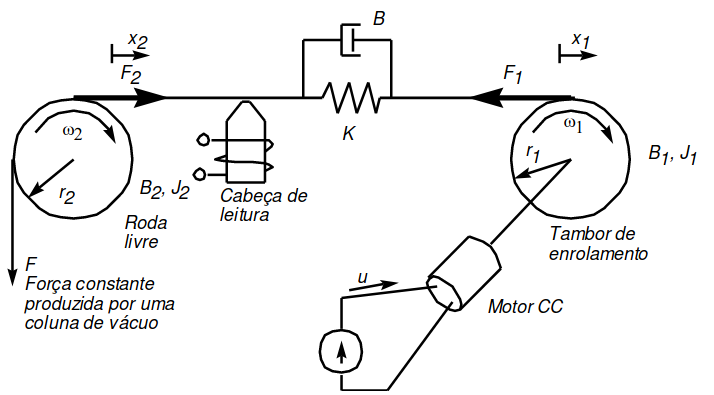
\includegraphics[width = 0.6\linewidth]{img/mechanics/motor-cc-P16.png}
    \caption{P16 retirado da coletânea de exercícios.}
    \label{fig:motor-cc-P16}
\end{figure}

\noindent\underline{T. de Enrolamento}: de acordo com as equações subjacentes à mecânica de rotação

\noindent \hspace*{1.5 em}\raisebox{0.2 em}{$\drsh$} $J_1 \dot{\omega_1} = - F_1 r_1 - \beta_1 \omega_1 + T_{cc}$

\vspace{0.5em}
\noindent\underline{Roda Livre}: novamente, de acordo com as equações subjacentes à mecânica de rotação 

\noindent \hspace*{1.5 em}\raisebox{0.2 em}{$\drsh$} $J_1 \dot{\omega_2} = (F_2 - F) r_2 - \beta_2 \omega_2$

\vspace{0.5em}
\noindent\underline{Fita}: (\textit{vide} \hyperref[def:MolasElásticas]{secção das molas elásticas})

\noindent \hspace*{1.5 em}\raisebox{0.2 em}{$\drsh$} $
                \begin{cases}
                    F_1 = K(x_1 - x_2) + \beta(\dot{x_1} - \dot{x_2})\\
                    F_2 = -K(x_2 - x_1) - \beta(\dot{x_2} - \dot{x_1})\\
                \end{cases}
$

\vspace{0.5em}
\noindent\underline{Motor CC}: $T_{cc}$ é o binário exercido pelo motor CC no Tambor de Enrolamento

\noindent \hspace*{1.5 em}\raisebox{0.2 em}{$\drsh$} $T_{cc} = K_T\, u$

\vspace{0.5em}
\noindent\underline{Variáveis do referencial}: a velocidade linear de um ponto da periferia de uma roda é o produto do raio da roda pela velocidade angular

\noindent \hspace*{1.5 em}\raisebox{0.2 em}{$\drsh$} $
                \begin{cases}
                    \dot{x_1} = \omega_1 r_1\\
                    \dot{x_2} = \omega_2 r_2\\
                \end{cases}
$

%//==============================--@--==============================//%
\clearpage
\paragraph[3.2.2.2 Problema 2]{$\pmb{\star}$ Escreva as equações que modelam o sistema e um modelo de estado na forma de um sistema de
equações diferenciais de 1ª ordem.}\mbox{}\\
\begin{figure}[H]
    \centering
    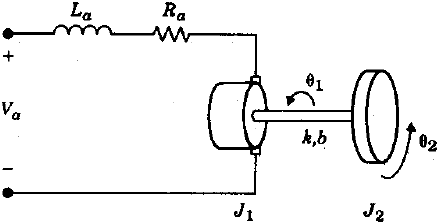
\includegraphics[width = 0.45\linewidth]{img/mechanics/motor-cc-P18.png}
    \caption{P18 retirado da coletânea de exercícios. Motor elétrico que reboca uma carga com um modo dominante de vibração.}
    \label{fig:motor-cc-P18}
\end{figure}

\noindent \underline{Motor:} por aplicação da Lei das Malhas (KVL)

\noindent \hspace*{1.5 em}\raisebox{0.2 em}{$\drsh$} \textbf{KVL}: $ L_a \dfrac{d i_a}{dt} + i_a R_a + e_a - V_A = 0 \iff \dfrac{d i_a}{dt} = -\dfrac{K_e}{L_a} \dot{\theta}_1 - \dfrac{R_a}{L_a} i_a + V_A$

\vspace{0.5em}
\noindent \underline{Veio:} com as equações subjacentes à mecânica de rotação

\noindent \hspace*{1.5 em}\raisebox{0.2 em}{$\drsh$} $J_1 \ddot{\theta}_1 = -K(\theta_1 - \theta_2) -\beta(\dot{\theta}_1 - \dot{\theta}_2) + T_{cc}$

\vspace{0.5em}
\noindent\underline{Motor CC}: $T_{cc}$ é o binário exercido pelo motor CC no veio

\noindent \hspace*{1.5 em}\raisebox{0.2 em}{$\drsh$} $T_{cc} = K_T\, i_a$

\vspace{0.5em}
\noindent \underline{Carga:} de acordo com as equações subjacentes à mecânica de rotação

\noindent \hspace*{1.5 em}\raisebox{0.2 em}{$\drsh$} $J_2 \ddot{\theta}_2 = -K(\theta_2 - \theta_1) -\beta(\dot{\theta}_2 - \dot{\theta}_1)$

\vspace{0.5em}
\noindent Definem-se então os estados: $\pmb{x} = \begin{bmatrix} \theta_2 & \dot{\theta}_2 & \theta_1 & \dot{\theta}_1 & i_a\end{bmatrix}^T$

$$
    \therefore \dot{\pmb{x}} = 
    \begin{bmatrix} 
        0 & 1 & 0 & 0 & 0\\[4pt]
        -\frac{K}{J_2} & -\frac{\beta}{J_2} & \frac{K}{J_2} & \frac{\beta}{J_2} & 0\\[4pt]
        0 & 0 & 0 & 1 & 0\\[4pt]
        \frac{K}{J_1} & \frac{\beta}{J_1} & -\frac{K}{J_1} & -\frac{\beta}{J_1} & K_T\\[4pt]
        0 & 0 & 0 & -\frac{K_e}{L_a} & -\frac{R_a}{L_a}
    \end{bmatrix}
    \pmb{x} +
    \begin{bmatrix} 
        0\\
        0\\
        0\\
        0\\
        -\frac{1}{L_a}
    \end{bmatrix}
    V_A
$$

%//==============================--@--==============================//%
\clearpage
\paragraph[3.2.2.3 Problema 3]{$\pmb{\star}$ Defina um estado apropriado com a menor dimensão possível e escreva as respetivas equações de estado na forma matricial. }\mbox{}\\
\begin{figure}[H]
    \centering
    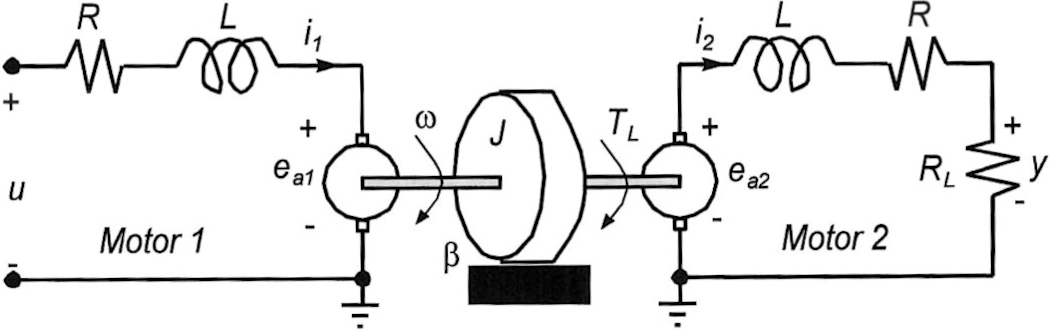
\includegraphics[width = 0.6\linewidth]{img/mechanics/motor-cc-exame2021.png}
    \caption{Circuito eletromecânico equivalente de dois motores de corrente contínua de íman permanente, que têm os veios ligados solidariamente. $T_L = K_T\, i_1$ e $e_{ai} = K_{ei}\, \omega$}
    \label{fig:motor-cc-exame20/21}
\end{figure}

\noindent \underline{Motor 1:} por aplicação da Lei das Malhas (KVL)

\noindent \hspace*{1.5 em}\raisebox{0.2 em}{$\drsh$} \textbf{KVL}: $i_1 R + L \dfrac{d i_1}{dt} + e_{a1} - u = 0 \iff \dfrac{d i_1}{dt} = - \dfrac{R}{L} i_1 - \dfrac{K_{e1}}{L} \omega + \dfrac{1}{L}u$

\vspace{0.5em}
\noindent \underline{Motor 2:} por aplicação, novamente, da Lei das Malhas (KVL)

\noindent \hspace*{1.5 em}\raisebox{0.2 em}{$\drsh$} \textbf{KVL}: $L \dfrac{d i_2}{dt} + i_2 R + i_2 R_L - e_{a2} = 0 \iff \dfrac{d i_2}{dt} = \dfrac{K_{e2}}{L}\omega - \left(\dfrac{R+R_L}{L}\right) i_2$

\vspace{0.5em}
\noindent \underline{Roda:} de acordo com as equações subjacentes à mecânica de rotação

\noindent \hspace*{1.5 em}\raisebox{0.2 em}{$\drsh$} $J \dot{\omega} = T_L - \beta \omega \iff \dot{\omega} = -\dfrac{\beta}{J}\omega + \dfrac{K_T}{J} i_1$

\vspace{0.5em}
\noindent Definem-se então os estados: $\pmb{x} = \begin{bmatrix} \omega & i_1 & i_2 \end{bmatrix}^T$

$$
    \therefore \dot{\pmb{x}} = 
    \begin{bmatrix} 
        -\frac{\beta}{J} & \frac{K_T}{J} & 0\\[5pt]
        -\frac{K_{e1}}{L} & -\frac{R}{L} & 0\\[5pt]
        \frac{K_{e2}}{L} & 0 & \frac{K_T}{J}
    \end{bmatrix}
    \pmb{x} +
    \begin{bmatrix} 
        0\\[5pt]
        \frac{1}{L}\\[5pt]
        0
    \end{bmatrix}
    u,\qquad y = 
    \begin{bmatrix}
        0 & 0 & R_L
    \end{bmatrix}
    \pmb{x}
$$

%//==============================--@--==============================//%
\clearpage
\subsection[3.2 Sistemas baseados em Mecânica Lagrangiana]{$\rightarrow$ Sistemas baseados em Mecânica Lagrangiana}
\label{sec:mechanics-lagrangian}

\phantomsection\addcontentsline{toc}{subsubsection}{3.2.1 Princípio de Hamilton}
\renewcommand*{\thefootnote}{\fnsymbol{footnote}}
\begin{theo}[\underline{Princípio de Hamilton} \cite{Maia2000}]{def:principio-hamilton}\label{def:principio-hamilton}
    De todo o conjunto de configurações admissíveis que um sistema pode assumir ao evoluir de uma configuração $1$ no instante $t_1$ para uma configuração $2$ no instante $t_2$, aquela que satisfaz as condições de equilíbrio dinâmico em cada instante é a que torna estacionário (mínimo) o integral da Lagrangiana\footnotemark[2] do sistema durante esse intervalo de tempo.
\end{theo}

\noindent ``Matematicamente, a condição de equilíbrio dinâmico corresponde a
$$
    \delta I = \delta \int_{t_1}^{t_2} (T-U) \, dt = \delta \int_{t_1}^{t_2} L \, dt = 0 
$$
em que $\delta$ representa a primeira variação de $I$. Não se trata de uma minimização clássica de uma função em relação a uma ou mais variáveis, pois das várias funções associadas às várias trajectórias possíveis, expressas pelo integral $I$, à sua minimização corresponde também uma função, que é a trajectória de equilíbrio. $I$ não é uma função, mas antes uma função de funções, que se designa por funcional.''\cite{Maia2000}
\noindent{\begin{center}\rule{8cm}{1pt} \end{center}} 

\footnotetext[2]{``\underline{\textbf{Note-se}} que a Lagrangiana, $L=T-V$, é uma medida do balanço entre a energia cinética e a energia potencial. Compreende-se, pois, que a integração no tempo dessa medida corresponde a uma situação de equilíbrio dinâmico.''\cite{Maia2000}}
\renewcommand*{\thefootnote}{\arabic{footnote}}

\noindent O princípio de Hamilton pode ser encarado como a integração no tempo do princípio dos trabalhos virtuais em dinâmica.

\begin{mdframed}
$$
    \therefore \int_{t_1}^{t_2} (\delta L + \overline{\delta W}_{\text{nc}}) \, dt = 0,\quad \delta r_i (t_1) = \delta r_i (t_2) = 0,\quad i = 1,\dots,N  
$$
\end{mdframed}
em que $\overline{\delta W}_{\text{nc}}$ representa o trabalho virtual das forças não-conservativas. Esta expres- são traduz o \underline{\textit{princípio de Hamilton generalizado}}\cite{Maia2000}.

\subsubsection[3.2.2 Equações de Euler-Lagrange]{$\rightarrow$ Equações de Euler-Lagrange}

É possível deduzir de uma forma muitíssimo elegante as equações de Lagrange através do princípio de Hamilton.

\begin{theo}[\underline{Equações de Euler-Lagrange} \cite{Maia2000}]{def:euler-lagrange}\label{def:euler-lagrange}
$$
    \frac{d}{dt}\left( \frac{\partial L}{\partial \dot{q}_k} \right) - \frac{\partial L}{\partial q_k} = Q_k,\quad k = 1,2,\dots,n
$$

\noindent em que $Q_k$ são as forças generalizadas não-conservativas.
\end{theo}

 \noindent ``Note-se que basta conhecer-se a Lagrangiana do sistema, que é um escalar, e as forças externas aplicadas, para---de uma forma directa---se obterem as equações de equilíbrio dinâmico. Naturalmente, a expressão indica que se obtêm $n$ equações, dado que o sistema tem $n$ graus de liberdade. ''\cite{Maia2000}

Se não existirem forças externas aplicadas, o sistema encontrar-se-á em movimento livre e a equação simplifica-se:
$$
    \frac{d}{dt}\left( \frac{\partial L}{\partial \dot{q}_k} \right) - \frac{\partial L}{\partial q_k} = 0,\quad k = 1,2,\dots,n
$$

%//==============================--@--==============================//%
\subsection[3.3 Sistemas Térmicos]{$\rightarrow$ Sistemas Térmicos}
\label{sec:mechanics-thermic}

Os sistemas térmicos dizem respeito ao aquecimento de corpos e ao transporte de energia térmica.

\begin{mdframed}
    A quantidade de calor $Q$ $[$J$]$ necessária para aquecer um corpo de massa $m$, levando-o de uma temperatura inicial $T_1$ à temperatura $T_2$, é dado por:
    $$
        Q = m c_p (T_2 - T_1)
    $$
    em que $c_p$ é o calor específico da substância de que é feito o corpo.
\end{mdframed}

\begin{mdframed}
    O fluxo de calor é dado por
    $$
        q = \frac{dQ}{dt}\; [\text{W}]
    $$
    O fluxo de calor afeta a temperatura de um corpo de acordo com
    $$
        \boxed{\frac{dT}{dt} = \frac{1}{C} q}
    $$
    \noindent em que $C = m c_p$ (em certos casos, a massa pode ser desconsiderada). Esta expressão obtém-se derivando a expressão que relaciona a quantidade de calor e a temperatura.
    \\[6pt]
    As \underline{equações diferenciais para a temperatura} obtêm-se contabilizando os \underline{fluxos} de calor \underline{que entram e saem} do corpo (conservação de energia).
\end{mdframed}

%//==============================--@--==============================//%
\subsubsection[3.3.1 Modos de transferência de energia]{$\rightarrow$ Modos de transferência de energia}

\paragraph[3.3.1.1 Transferência de energia por condução]{$\pmb{\star}$ Transferência de energia por condução}\mbox{}\\
Um corpo (a $T_2$) encostado a outro com temperatura inferior, transfere energia para este com fluxo de calor dado por:  
$$
    \text{\underline{Lei de Fourier}:}\quad \boxed{q = \frac{1}{R} (T_2 - T_1)}
$$
\noindent em que $R$ $[$$^{\circ}$C/J/s$]$ é a resistência térmica.

\vspace{-1em}
\paragraph[3.3.1.2 Transferência de energia por convecção]{$\pmb{\star}$ Transferência de energia por convecção}\mbox{}\\
A transferência de energia por convecção está associada ao transporte de massa num fluido que se desloca. Por vezes é razoável assumir (não existe um modelo geral simples):
$$
    q = c_r (T_2 - T_1),\qquad c_r \in \mathbb{R}
$$

\vspace{-1em}
\paragraph[3.3.1.2 Transferência de energia por radiação]{$\pmb{\star}$ Transferência de energia por radiação}\mbox{}\\
Um corpo à temperatura absoluta $T$ $[$K$]$ radia uma potência $q$ $[$W$]$ dada pela lei de Stefan-Boltzman:
$$
    q = A \varepsilon \sigma T^4
$$
onde $A$ $[$m$^2]$ é a área de exposição do corpo; $\varepsilon \in [0,1]$ a emissividade do corpo; e $\sigma$ a constante de Stefan-Boltzman ($\sigma = 5.670374419\hdots \cdot 10^{-8}$ $[$Js$^{-1}$m$^{-2}$K$^{-4}]$). 
%//==============================--@--==============================//%